\documentclass[11pt]{article}

\usepackage{changepage}
\usepackage{graphicx}
\usepackage{amssymb} %math symbols
\usepackage{mathtools} %more math stuff
\usepackage{amsthm} %theorems, proofs and lemmas
\usepackage{optidef} %fast optimization problem notation
\usepackage{biblatex} %Imports biblatex package
\addbibresource{papers.bib} %Import the bibliography file

%% declaring abs so that it works nicely
\DeclarePairedDelimiter\abs{\lvert}{\rvert}%
\DeclarePairedDelimiter\norm{\lVert}{\rVert}%r

\title{MICRO-502 - Aerial Robotics Project}
\author{Filip Slezák, Jean Lesur, Titouan Renard}

\begin{document}

\maketitle

\section{Introduction}



\subsection{Presentation of the Crazyflie platform}

\subsection{Problem statement and discussion of possible pitfalls}

\begin{figure}[h!]
    \centering
    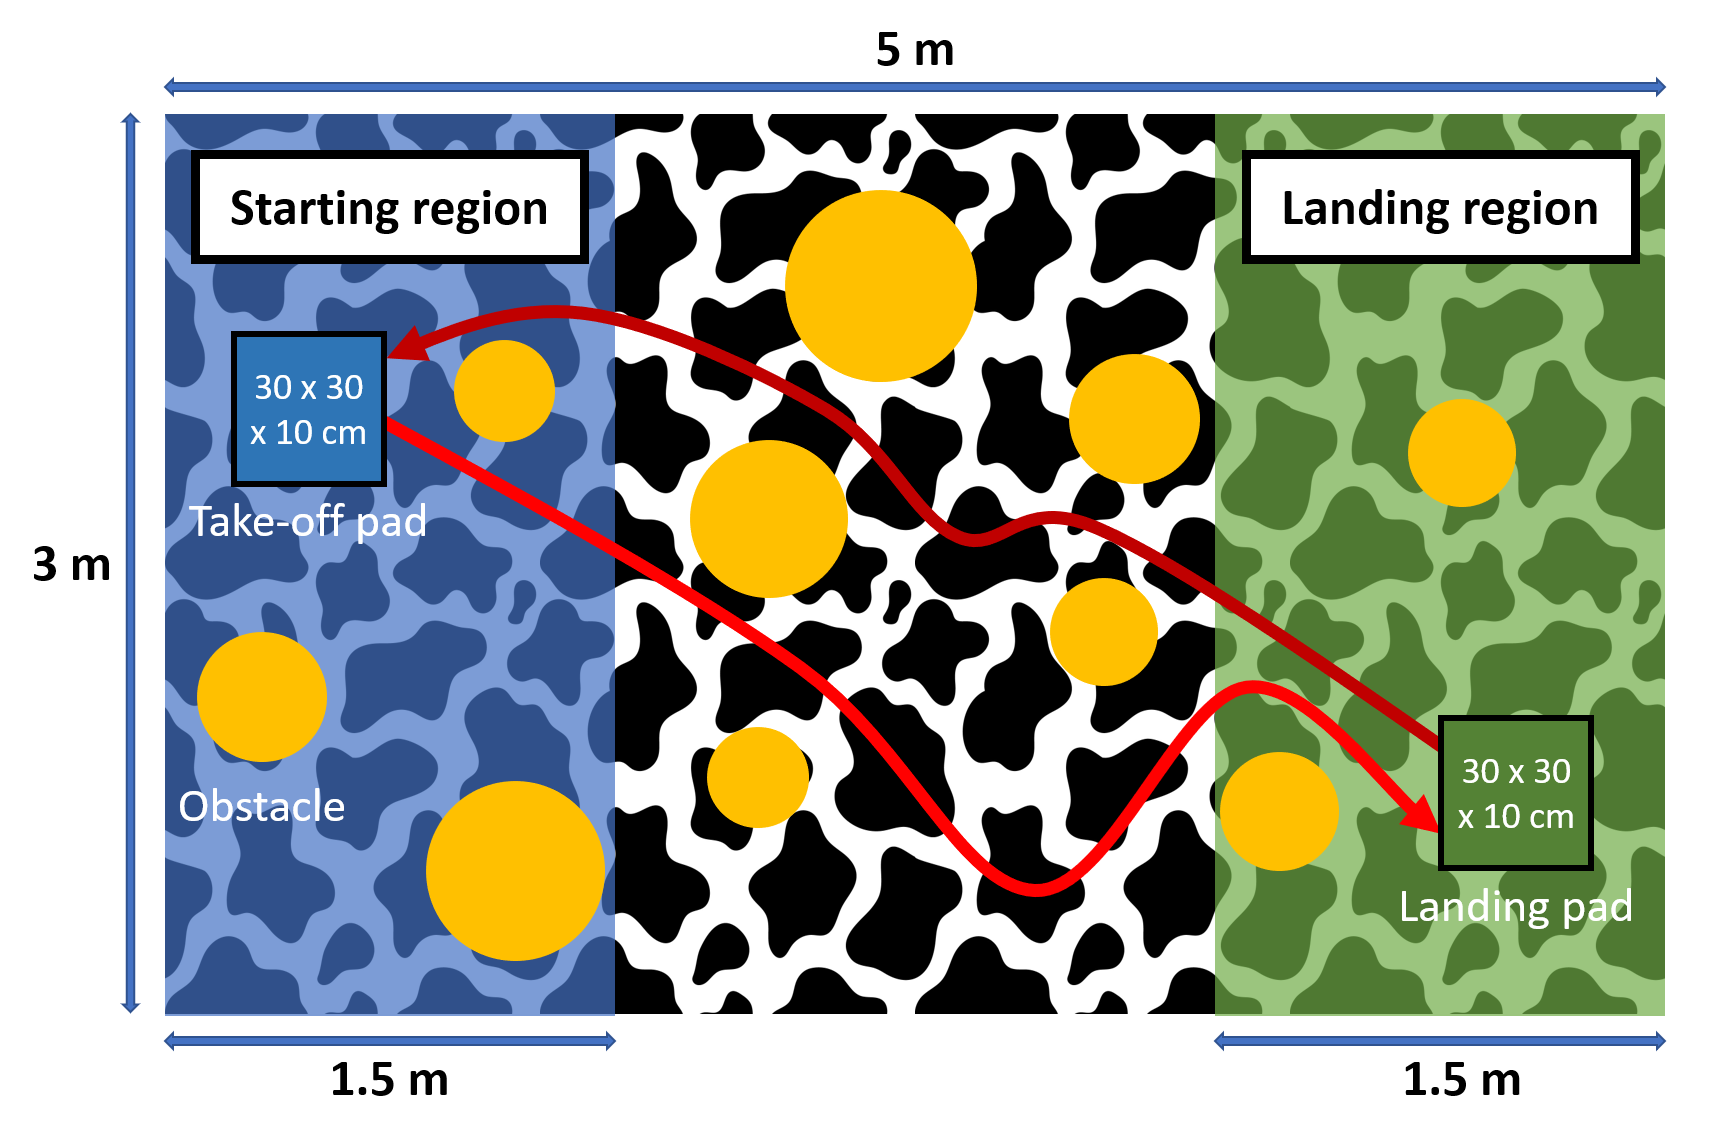
\includegraphics[width=0.8\textwidth]{figures/crazyfly_objective_figure.png}
    \caption{Schematic representation of the flight area.}
\end{figure}

\section{General presentation of our solution}

\begin{figure}[h!]
    \centering
    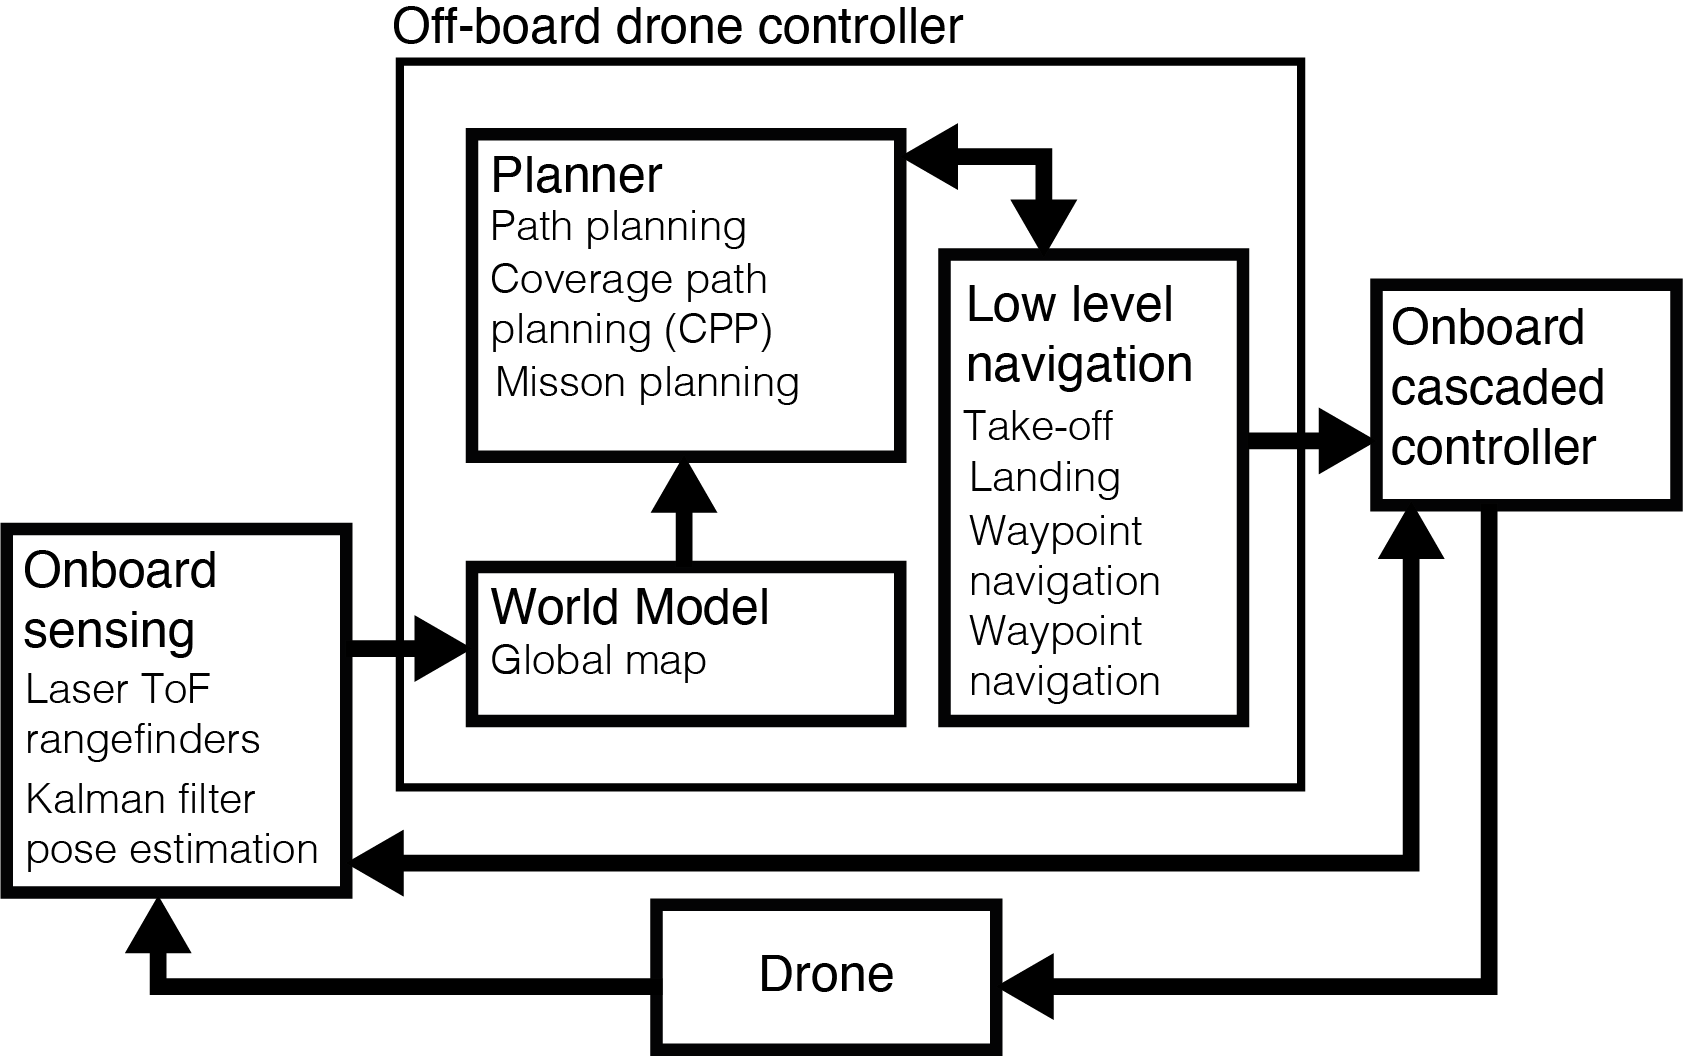
\includegraphics[width=0.7\textwidth]{figures/arch.png}
    \caption{Schematic representation of the hybrid architecture.}
\end{figure}

Our software implements a hybrid-deliberative architecture that can be split into three main components :
\begin{enumerate}
    \item an off-board deliberative \textit{supervisor} that maintains a world model (a map) and ensures the planning of actions,
    \item an off-board low level \textit{controller} that performs navigation tasks (such as take-off, landing and waypoint navigation).
    \item an on-board control system and state estimator that handles control of the robot.
\end{enumerate}


\section{World model and path planning}

In the following section we present the design of the deliberative agent that handles path planning and mission planning. We call mission planning ensuring that the robot achieves its specified goals (in our case taking off platform $A$, flying and landing on platform $B$ and going back to platform $A$). Our supervisor agent can be split up into two main components : 
\begin{enumerate}
    \item a mission-planner finite state machine that handles mission planning,
    \item a path planner component that handles global navigation and implements two distinct path planning algorithms : 
    \begin{enumerate}
        \item an online shortest path path planing algorithm,
        \item an online coverage path planing algorithm.
    \end{enumerate}
\end{enumerate}

Both path planning algorithms rely on a global nav that is updated in realtime according to the sensor values. Those different components are described separately in the section below.


\subsection{Mission-planner finite state machine}

\subsection{World representation : online mapping with uncertainty}

\subsection{Online path planing}

\textbf{TODO : Write that and explain the procedure} \textit{What we do can be though of a a really rough (and discretized) perception aware path planing algorithm.}

\subsection{Coverage path planning}

\cite{epsilon_star} \cite{Galceran13asurvey} \cite{recsplit}

\section{Low level navigation}

\section{Results}

\section{Conclusion}

\tableofcontents

\printbibliography %Prints bibliography

\end{document}
